\Subhead{1.4.4}{Анализ возможных движений и бифуркаций в фазовом пространстве}
\textbf{Фазовое пространство} состоит из состояний системы; для автономного осциллятора это $(x,v)$, $\dot x=v$, $\dot v=F(x,v)$. Векторное поле задаёт направление движения. При единственности решений траектории в полном фазовом пространстве не пересекаются. Для периодически вынужденной системы надо добавить фазу воздействия: проекции на $(x,v)$ пересекаться могут.

У равновесия $\bm z_*$ линеаризация $\delta\dot{\bm z}=J\delta\bm z$ даёт показатели $\lambda$. Седло имеет направления притяжения и отталкивания, узел --- вещественные показатели одного знака, фокус --- комплексную пару с ненулевой действительной частью. Отрицательные действительные части дают притяжение. Чисто мнимые показатели нелинейной задачи \emph{не доказывают центр}: нужен анализ нелинейных членов или интеграл энергии.
\begin{center}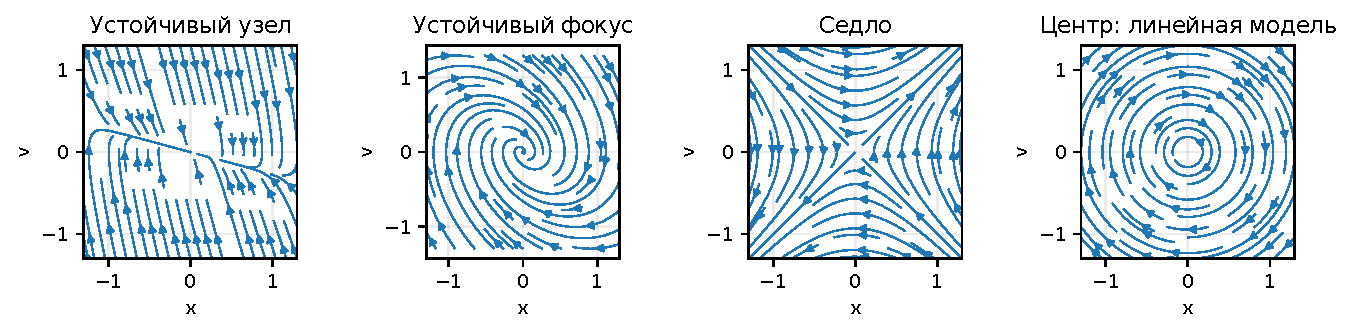
\includegraphics[width=.96\linewidth]{figures/phase_portraits.pdf}\end{center}
Предельный цикл --- изолированная периодическая орбита; сепаратрисы отделяют разные типы движения. Например, у консервативного маятника уровень энергии через верхнее равновесие отделяет качания от вращений. Семейство эллипсов линейного осциллятора не является семейством предельных циклов.

\textbf{Бифуркация} --- качественная перестройка движений при изменении параметра; это объект исследования, а не ещё один вариант гармонического баланса. Два основных примера:
\begin{itemize}
\item $\dot x=\mu-x^2$: при $\mu>0$ есть устойчивое $+\sqrt\mu$ и неустойчивое $-\sqrt\mu$ состояния; при $\mu=0$ они сливаются, затем исчезают. Это седло-узловая бифуркация; аналог --- край захвата фазы.
\item $\dot r=\mu r-br^3$, $\dot\theta\simeq\omega_*$, $b>0$, $\omega_*\ne0$: при пересечении $\mu=0$ рождается устойчивый цикл $r=\sqrt{\mu/b}$. Это сверхкритическая бифуркация Андронова--Хопфа, связанная с мягким возбуждением. Подкритический малый цикл неустойчив; большой устойчивый цикл и гистерезис требуют дополнительных нелинейных членов.
\end{itemize}
Для периодического режима строят отображение Пуанкаре; неподвижная точка отвечает циклу. По изменению его мультипликаторов различают складку циклов, удвоение периода и рождение тора (\Qref{1.8.2}, \Qref{1.11.2}). Качественный анализ начинают с равновесий, нульклин и направления поля, затем проверяют устойчивость и перестройки. Нульклина не обязана быть траекторией.
